This section enters in more details for specifically aspects in the implementation of each client and the back-end.

The next snippet code contains the rule to access the database.  Thus, to read and write in the data base, the authentication process must be succeeded, otherwise is not possible to have access for these two basic functionalities. This is the way to keep suavely the user's information, while security connection is guaranteed with HTPPS through Firebase.

\begin{figure}[ht]
\centering
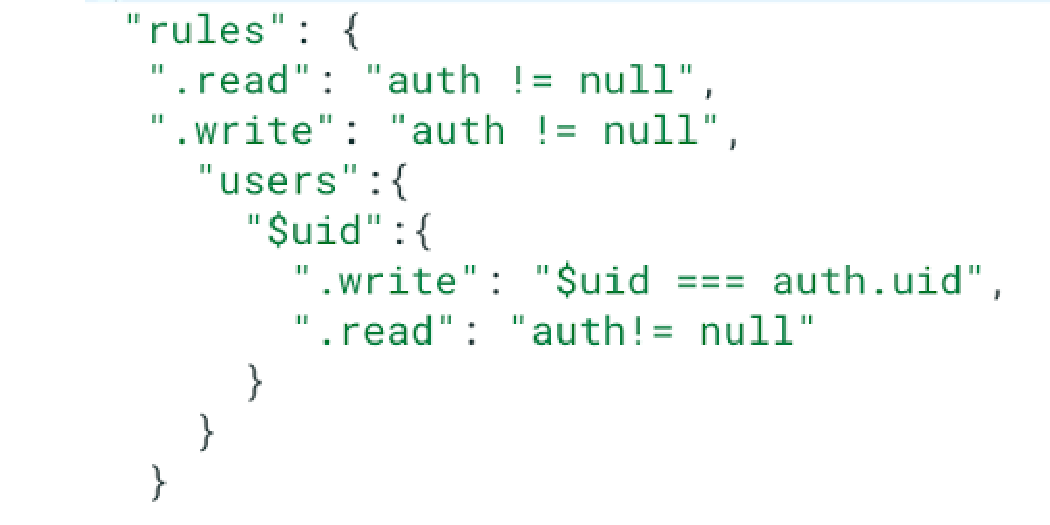
\includegraphics[width=0.5\textwidth]{figs/databaserules}
	\caption{Database Rules}
	\label{fig:databaserules}
\end{figure}

\subsection{iOS Implementation}

Figures 4 and 6 present the specific architecture and database interaction of the iOS client.

\begin{figure}[ht]
\centering
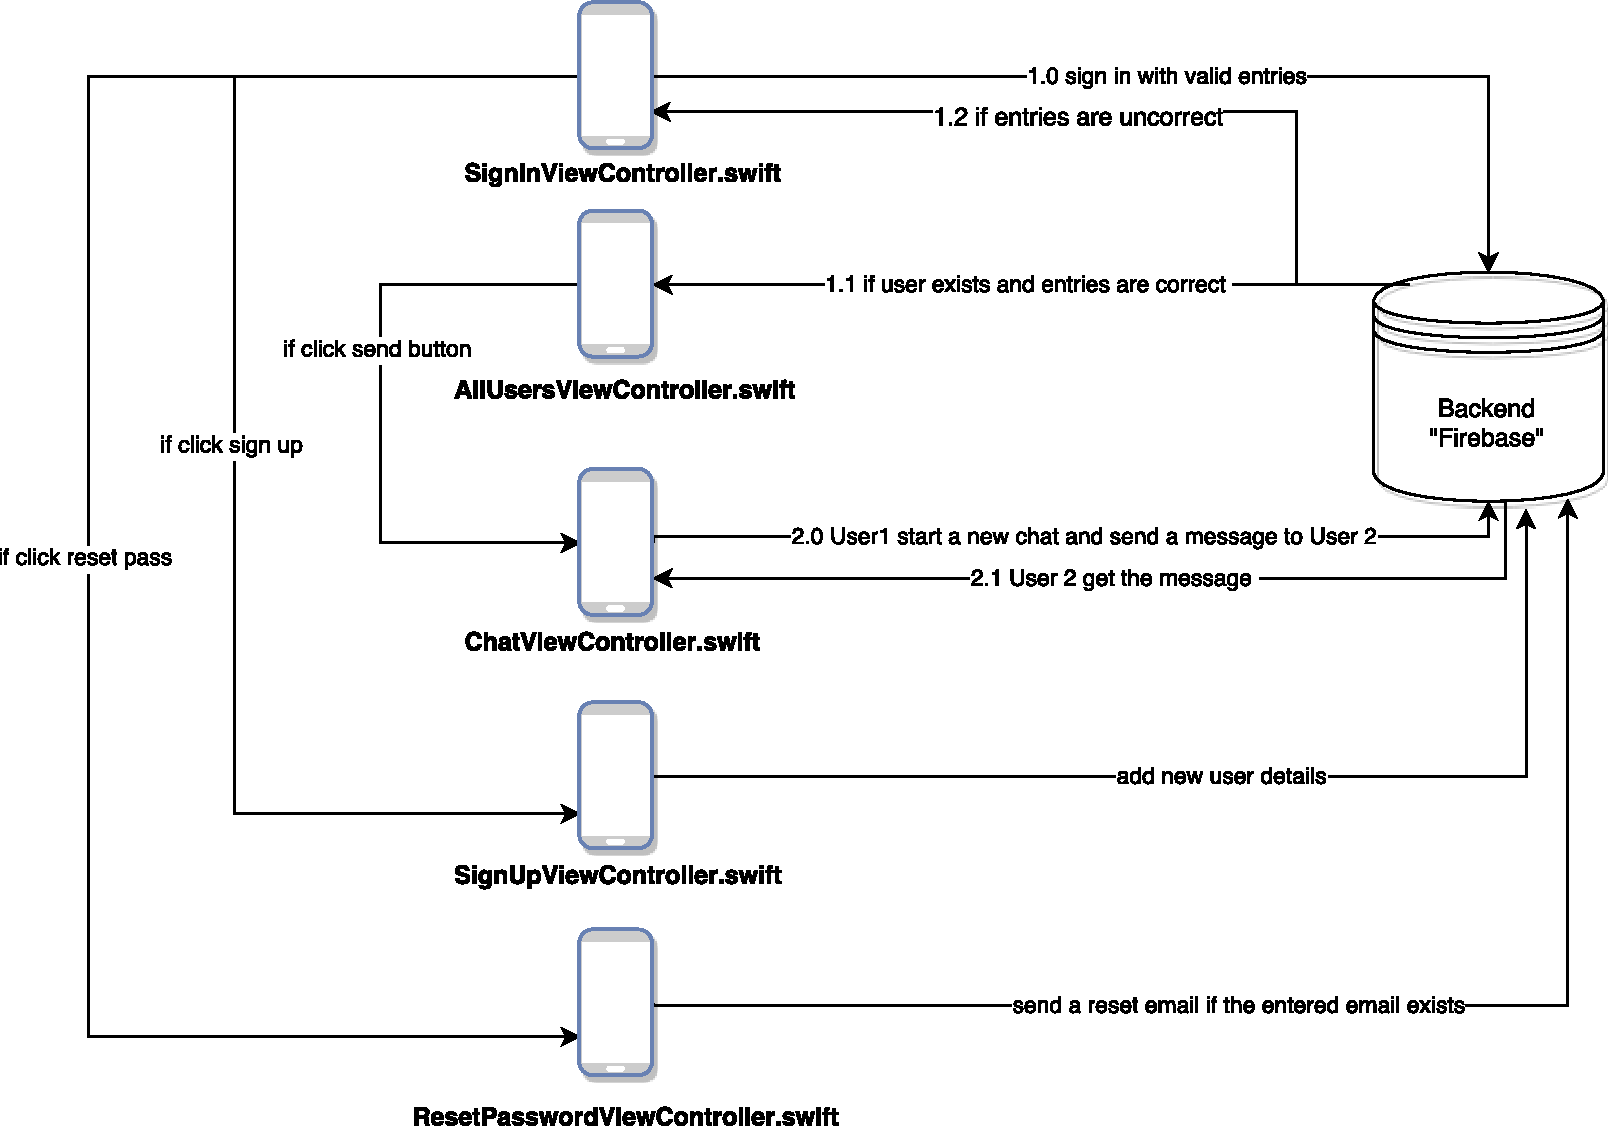
\includegraphics[width=1\textwidth]{figs/iOSarchitecture}
	\caption{iOS Database Interactions}
	\label{fig:iOSarchitecture}
\end{figure}
\textbf{Achievements and Challenges}: The iOS client was able to carry out all the tasks listed under Priority 1 successfully. However, some of the most challenging aspects were how to fetch users and check if the users have chatted before.

\begin{figure}[ht]
\centering
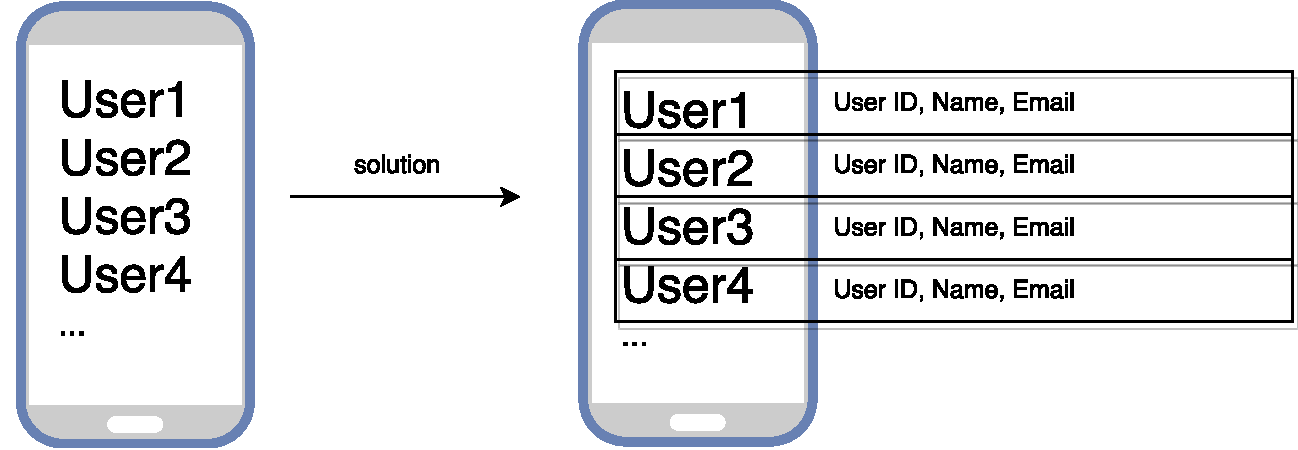
\includegraphics[width=0.75\textwidth]{figs/iOS_fetch_users_ID_issue_and_solution}
	\caption{Fetching Users in iOS}
	\label{fig:iOS_fetch_users_ID_issue_and_solution}
\end{figure}

Some of the most relevant specific details across iOS development and stated in the next subsections.   

\textbf{Fetch users}: The sender must ensure that the sent message go only to the intended receiver using the first UI (left side in Figure 7). To resolve this, we fetch the data of users as an array of array (as shown in the UI on the right of Figure 7) from the back-end to have the ID of the selected user.

\begin{figure}[ht]
\centering
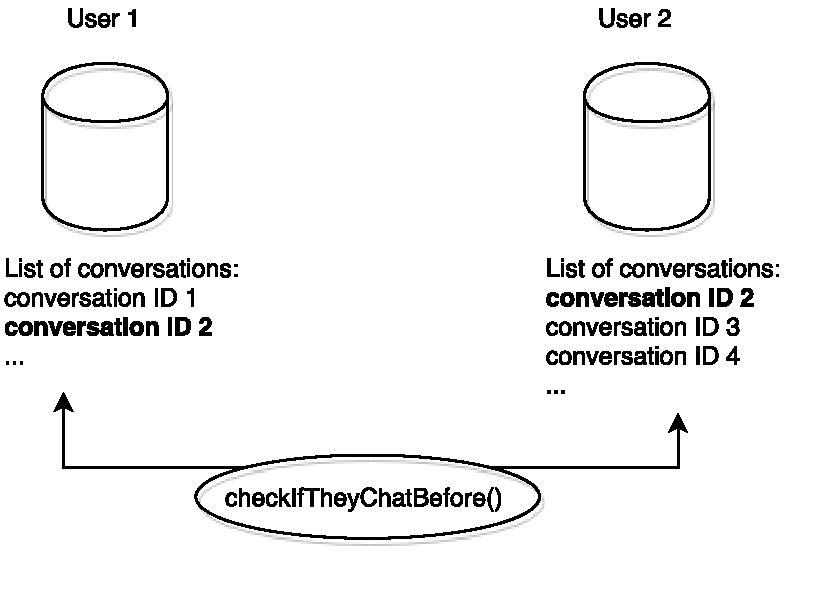
\includegraphics[width=0.6\textwidth]{figs/iOS_check_if_they_chatted_before}
	\caption{Helper function to check if chat exists}
	\label{fig:iOS_check_if_they_chatted_before}
\end{figure}

\textbf{Check if they chatted before}: When the user is trying to set up a new chat, it was difficult to find out if there is a previous chat with the receiver. There were several attempts made using different approaches to figure out a solution. Finally, we were able to come up with a function that carries out the logic shown in Figure ~\ref{fig:iOS_check_if_they_chatted_before}). Once a user (User1) selects another user (User2) to chat with, the function checkIfTheyChatBefore() compares the IDs of conversations from both sender and receiver records.  If there exist a common ID, then it implies that they had chatted before and the same conversation ID is used to store messages. Otherwise, a new conversation is created in the database.

\textbf{External Library}: We used two libraries namely; UIKit and CocoaPods. UIKit is a library already integrated in xCode which was used to make text fields, buttons, labels, and tables. However, using Cocoa Pods is mandatory for Firebase as a back-end.

\textbf{Code by others}: We use a code written by @Esqarrouth from http://stackoverflow.com/ to write the function hideKeyboardWhenTappedAround() in SharedFunc.swift (Github: Whisper/iOS/iOS/) which hide the keyboard when user taps anything else on the screen other than the keyboard.

\subsection{Web Implementation}

The WhatsApp Web Client was a great inspiration for us. Some of the key aspects of our web app are as follows. For the registration, we use a small plug-in called FirebaseUI that helps us connect with Firebase and select the providers we want to choose. We used Mail, Google and Facebook because those are the most popular.

For the whole App Wrapper, we used React JS which is a JavaScript Library developed by Facebook. React basically works as a multi component oriented framework that aims to simplify the logic of web applications by making apps more modular. It handles all the information, including user interface state in a state object that can be shared with other components or a local state only available to itself. After some event occurs, react re-renders the changed component to reflect the new state. Along with it, we learn the hard way that a Chat application needs a lot of rendering of elements in both direction (from parent to children and backwards). Therefore, we struggled a lot and we changed our main objective by doing some research and finding out that precisely, a lot of developers had the same problem when dealing with these type of applications. They were communicating bidirectionally between parents and children in the DOM Tree way too many times. That's how we learnt that Whisper was an excellent use case for Redux. 

Redux is another library that dispatches actions from the user interface to a reducer, which in turn sends the new state to the store (which is a global state for the app). Also with this, we learned the hard way that Redux couldn't manage asynchronous calls to a server by itself. Therefore, we used a middleware called Redux-thunk which takes care of this by simply dispatching actions on demand. That is, dispatch an action when we finished, for instance, fetching elements from Firebase.

Finally, for the styling we used stylus, CSS, and Bootstrap alpha 4 to accelerate our development and learn the newest trends in the front-end development community.

It is important to mention that we learned a lot of web development thanks to this project. We focused in these technologies because they are among the most used online in communities like Stack Overflow, Hacker News, and Reddit Web Development related subreddits.

Contrasting with iOS and Android, there are so many options out there to begin Web App Development. Being objectively, HTML and CSS are just not enough for this kind of project. As we know, HTML only serves the purpose of giving the structure to the web. That is, structuring all the information inside the DOM hierarchically and in order, tag by tag and element by element. As the name suggests CSS (Cascading Style Sheets), give the style or appearance to each HTML tag inside the DOM, properties such as position, colour, font weight, variant and sizes, background images, padding, margin, etc., are the ones that CSS controls so users can have a much better experience. 

However, we knew that this project was going to be heavy on the scripting side; we started looking out for technologies to take our development to the next level. Some of our research suggested that we used a powerful framework that took care of the rendering of elements almost in real time. To take advantages of the asynchronous functionality of Firebase, we decided to try it with the following various contestants: Vanilla JavaScript, AngularJS, ReactJS, jQuery and Ember.

Pure JavaScript is always needed for every heavy front-end development app, because that's the scripting part of it. However, pure JavaScript can lead to messy code and just recently with ES6 and ES7, with modular exports, is getting more friendly towards heavy applications, as we know. Although we are not experts at all and some of us have a little bit more experience using Python and Django for Back-End software development, we see a lot of resemblance between JavaScript classes and exports with Django Class Views.

AngularJS was an attractive option, is powered by Google and we consider this as a plus. Also, there are tons of material out there to learn, from community blog posts and books to complete courses on Coursera. On the other hand, jQuery is a JavaScript Library that has been out there since 2006, and although front-end frameworks change continuously  ~\ref{fig:5656rtyrt}, we learnt that jQuery was a leader at the time and still, for some basic stuff like AJAX is the go to for full-stack developers. 

React, being developed by Facebook, has a really strong community and hype around Internet blogs and the Stack Overflow Community Survey of 2017 ~\ref{fig:DeveloperStackoverflow}, however we didn't knew the potential until we read the well written documentation of it.

React's documentation, ease of use and hype, gave us the confidence to pick it up as a great library/framework to learn from. That's why we choose it for the Web Client development. React is used mainly by experienced software engineers in the front-end development industry. React facilitates most of the job on front-end development because it suggests to create your web applications using components for each task that needs to be done by your app, however that doesn't make it easy. Treating every bit of it as an isolated component that can even be reused on different future apps is the main benefit against others. The scope of these components is to focus on doing an specific task to make your application easier to understand to other developers. 

React is a little bit intimidating, some of the information out there can be confusing because to develop for it you need a little extra setup. Not like iOS or Android which only need Xcode and Android Studio respectively.

In contrast, you need to install NodeJS, npm (included) and Babel to transpose JavaScript newest syntax for older browsers. Additionally, they always suggest to use Gulp or Grunt to create tasks that automate a lot of the repetitive and tedious tasks inside front-end development such as compiling the different JavaScript source files, merging together all the CSS or style files, and running web pack to refresh your website with hot reloading whenever a new change is detected (basically to avoid refreshing the browser window).

All these tools that we have just mentioned are just needed for the development. For the actual code to make its job and suggested by React inside their documentation, they advise to use JSX, which is basically a way of writing JavaScript and HTML inside your JavaScript files.


\begin{figure}[ht]
\centering
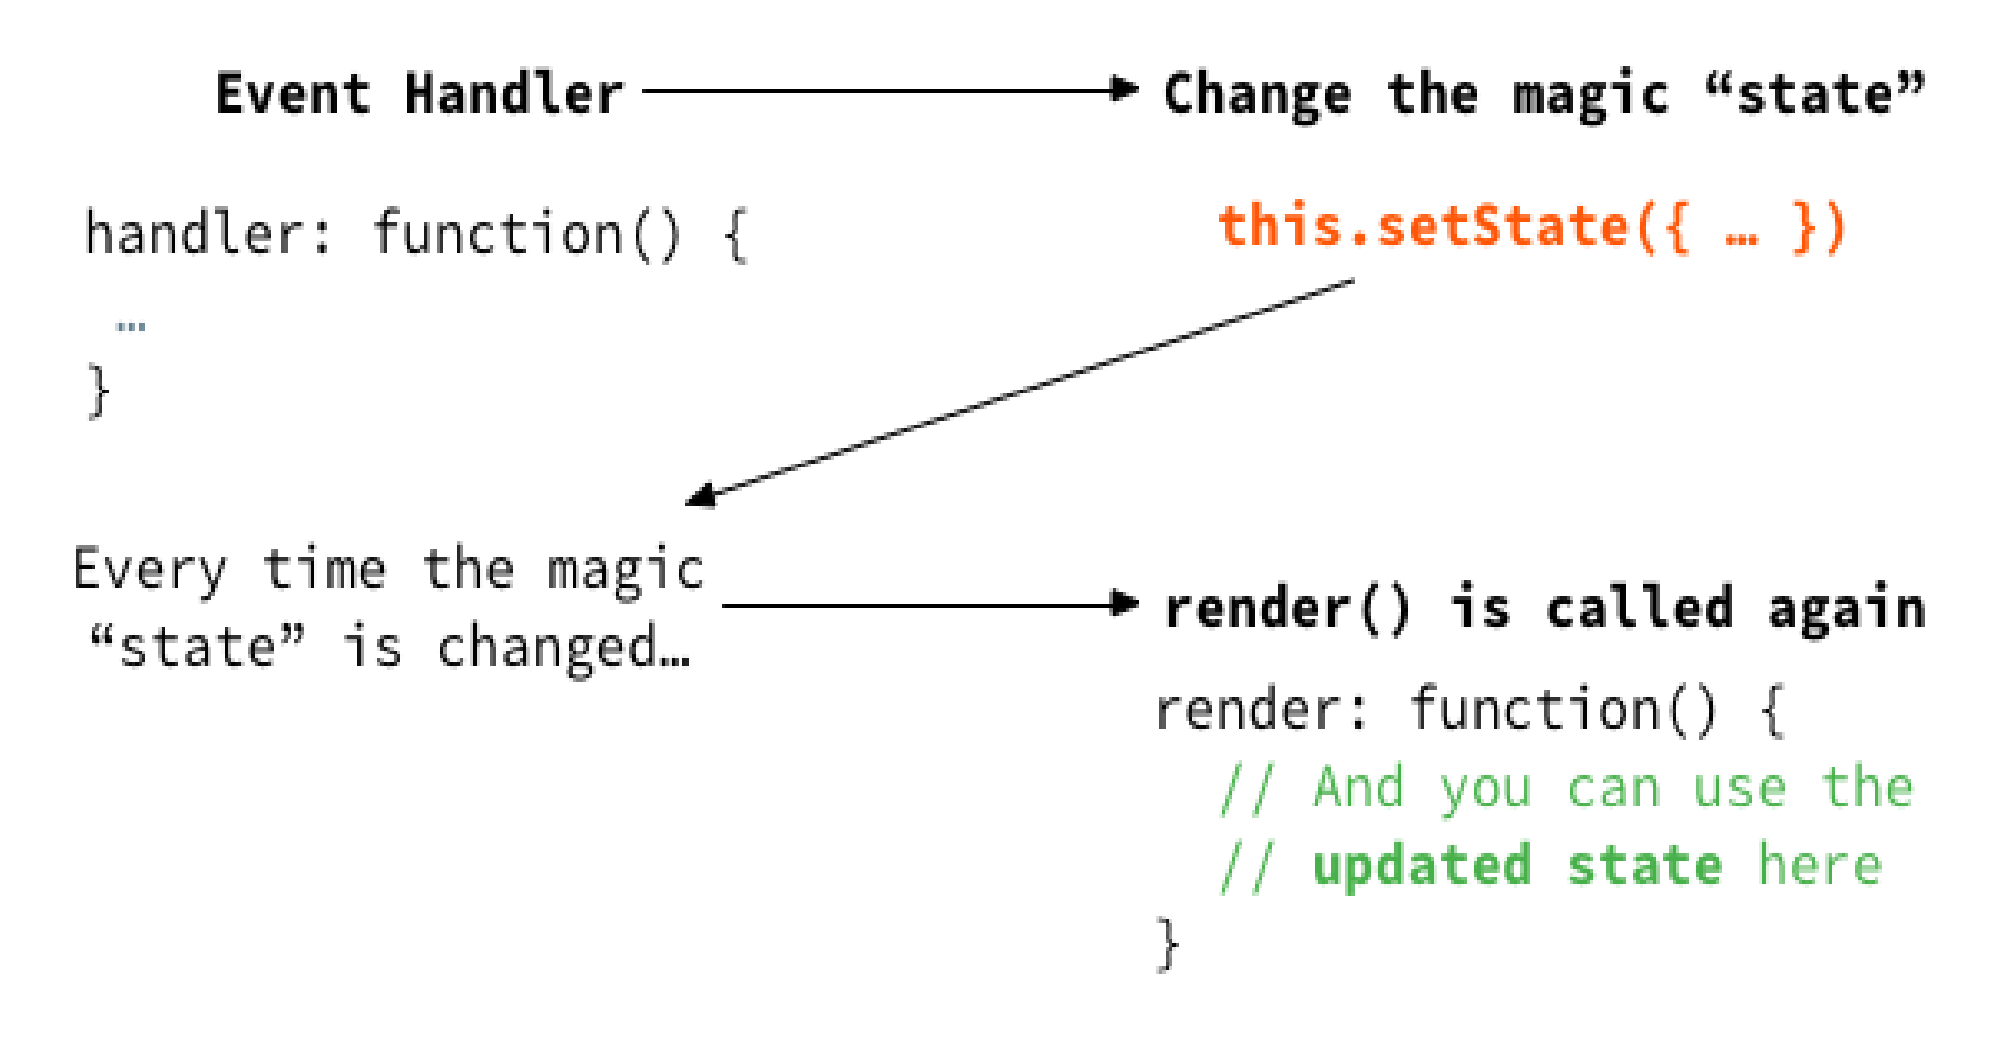
\includegraphics[width=0.6\textwidth]{figs/reactstyle}
	\caption{Overview React State and Render}
	\label{fig:reactstyle}
\end{figure}

Modular components and state are the most important aspects behind React development. For our case, it was very useful because our code was structured this way to achieve way more readability (on most of the cases) and to think about the big picture easily. And state management was very helpful because we could see state in real time thanks to the Chrome React extension. By this, the debugging process is less painful and much more friendly.

Some aspects of JavaScript language specifically made us struggle a lot, mainly because we did not have enough experience but mostly because of the ES5/ES6/ES7 standards and the way some documentation refer to their best-practices. That is why many people suggest using a library called Babel which was created by one of Facebook's employee ~\cite{4646eyyeye}.

This library, among other capabilities, gives the developer the ability of using fat arrow functions and in general features that are not yet available in some browsers:

\begin{figure}[ht]
\centering
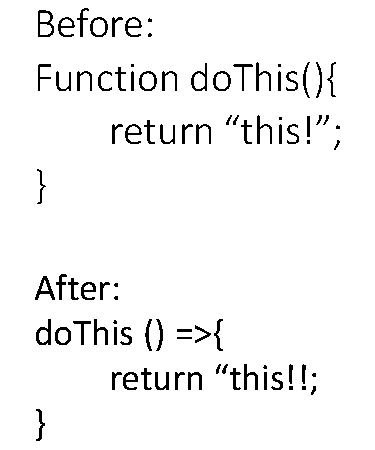
\includegraphics[width=0.2\textwidth]{figs/before}
	\caption{Fat Arrow Functions in JS}
	\label{fig:before}
\end{figure}

Some of these features of the JavaScript programming language gave us difficulties. One problem that really complicated things was the “this” keyword in our functions. Apparently in JavaScript this is not the same as, for example, “self” keyword in Python. More on that later when we explain Firebase integration.

In React, we opted to have the following main components which can be found inside the components directory:



\begin{enumerate}
	\item \textbf{AppWrapper}: The whole container wrapping all the components together and passing the state from Redux (more on that below) to the rest of the components.
	\item \textbf{ConversationsSidebar}: To render on the left side of the app, the conversations that each user have.
	\item \textbf{ConversationPanel}: The right-side panel that shows all the messages sent between users inside the selected conversation of the ConversationSidebar.
	\item \textbf{UserDrawer}: In charge of showing all the users available inside our application in the Users JSON (except the current logged user).
	\item \textbf{AddMessage}: This is the main component that takes care of dispatching most of the logic whenever is triggered. This is the main form element that adds the message to the Messages, Conversations, and Participants JSON when needed.
					
\end{enumerate}


We used Redux, because at first we tried it the hard way. We were using pure React to develop our app but because in react you must pass all the state from the parents all the way through the children that needs that piece of state, code can get chaotic. The following image illustrates how Redux solves a lot of the passing props from one side to another by using an independent store that handles all the data.

\begin{figure}[ht]
\centering
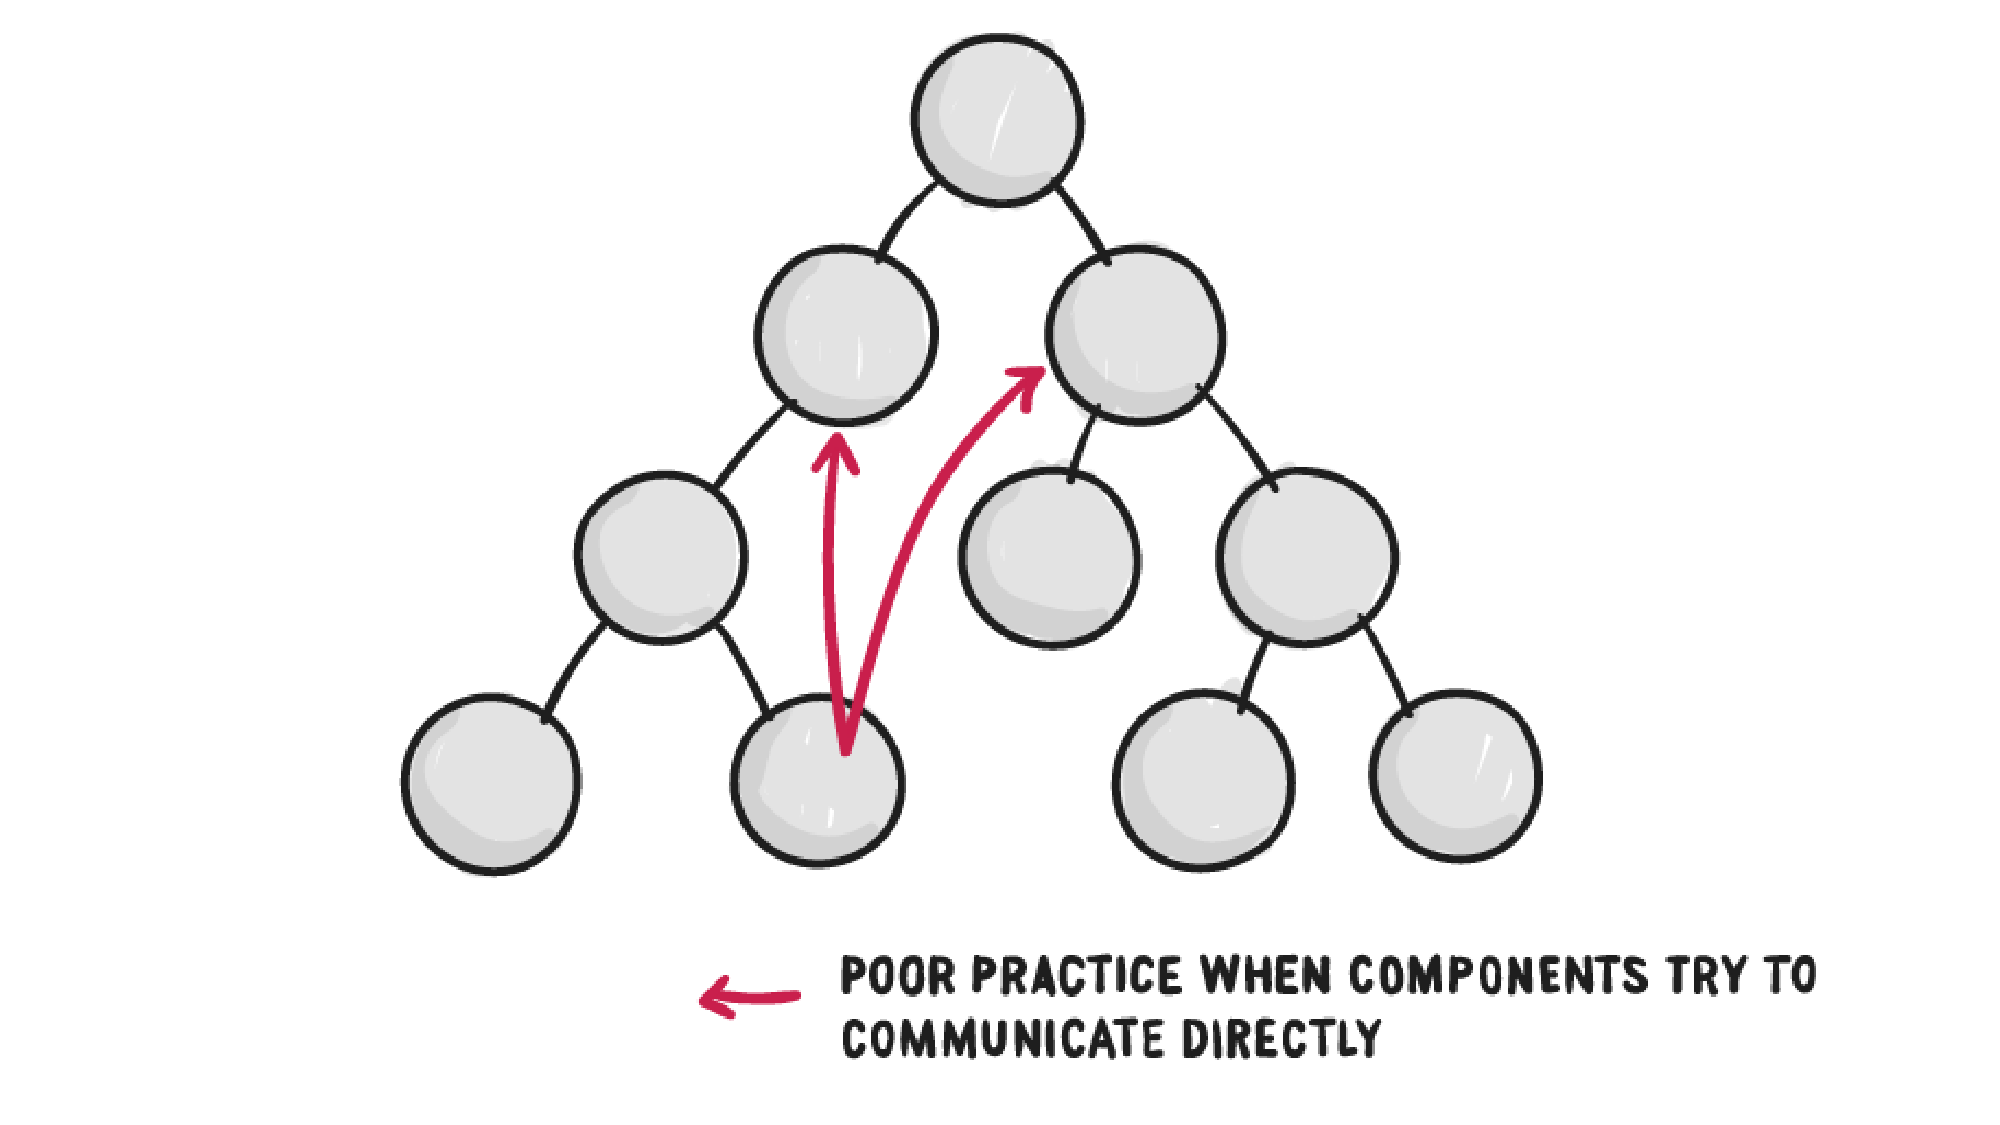
\includegraphics[width=0.5\textwidth]{figs/poorpractice}
	\caption{Hard to do when app gets complex}
	\label{fig:poorpractice}
\end{figure}


\begin{figure}[ht]
\centering
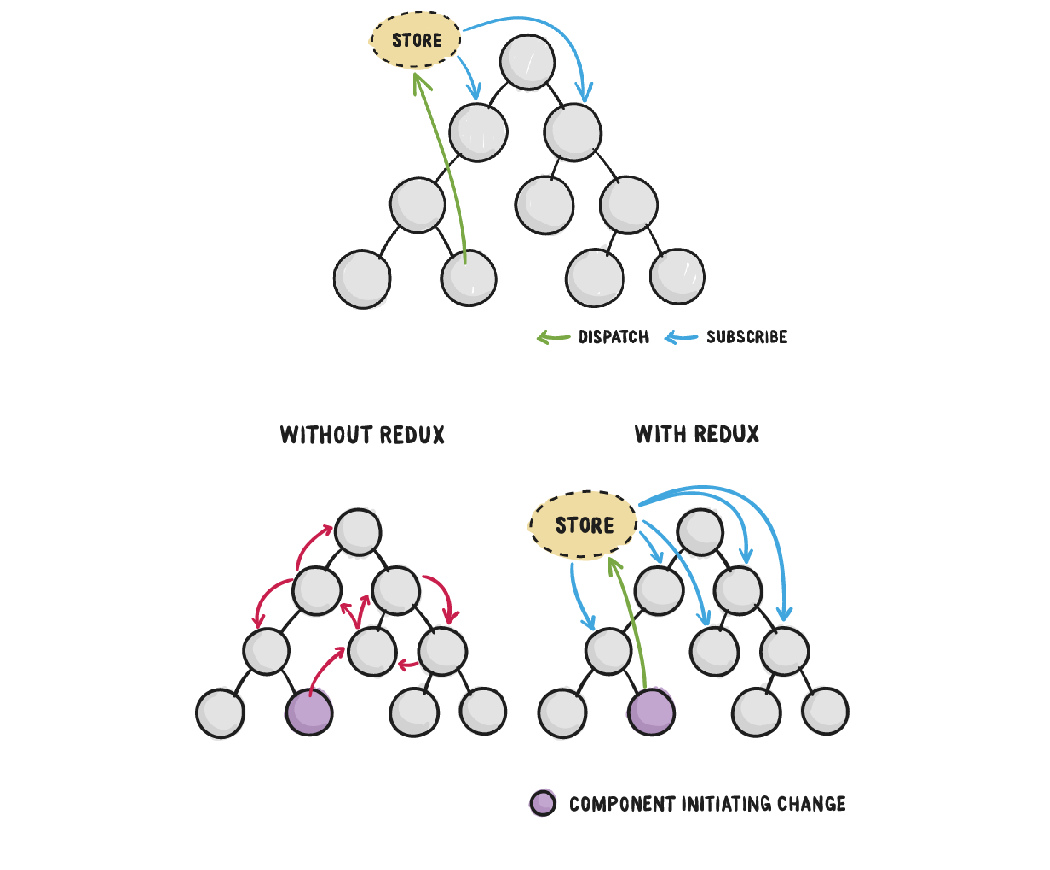
\includegraphics[width=0.5\textwidth]{figs/rtrtrtryeyeyeye}
	\caption{How Redux solves this}
	\label{fig:rtrtrtryeyeyeye}
\end{figure}

We were advancing with the application when we realised that code started to get complicated. That’s why in our commit history we show a drastic change of code from non Redux to it.
Using Redux was not as easy as we thought. The theory behind it is simple, use a store that holds all your app state (conversations, users, messages, and participants), fill that state when needed by using Actions and Dispatchers and then return the modified state with the Reducers.
Actions is a very simple concept, every time something happens in the client, an action is dispatched. When this action is dispatched, all the reducers listen, if they “own” the given action, then they update the state accordingly. One of the most important parts of Redux is that Reducers need to be pure functions.
The whole state of your app is stored in an object tree inside a single store.
The only way to change the state tree is to emit an action, an object describing what happened. We write reducers to specify how the actions transform the state tree ~\cite{ryryyrt346}.

Pure functions mean that you should not mutate the state object, but return a new object if the state changes. This is tricky at first and we ended up making a lot of mistakes on the first implementation, however, React and Redux documentation explain it well, however we didn't understand it. Which resulted in these errors of strange behaviour between state changes.

All our logic for Reducers was added to a folder called Reducers. The same thing for Actions, all are inside the actionCreator.js and the Constants for it are on the file with the same name.

The next Figure ~\ref{fig:actions-states} explains how our Whisper Web Client handles actions and state.


\begin{figure}[ht]
\centering
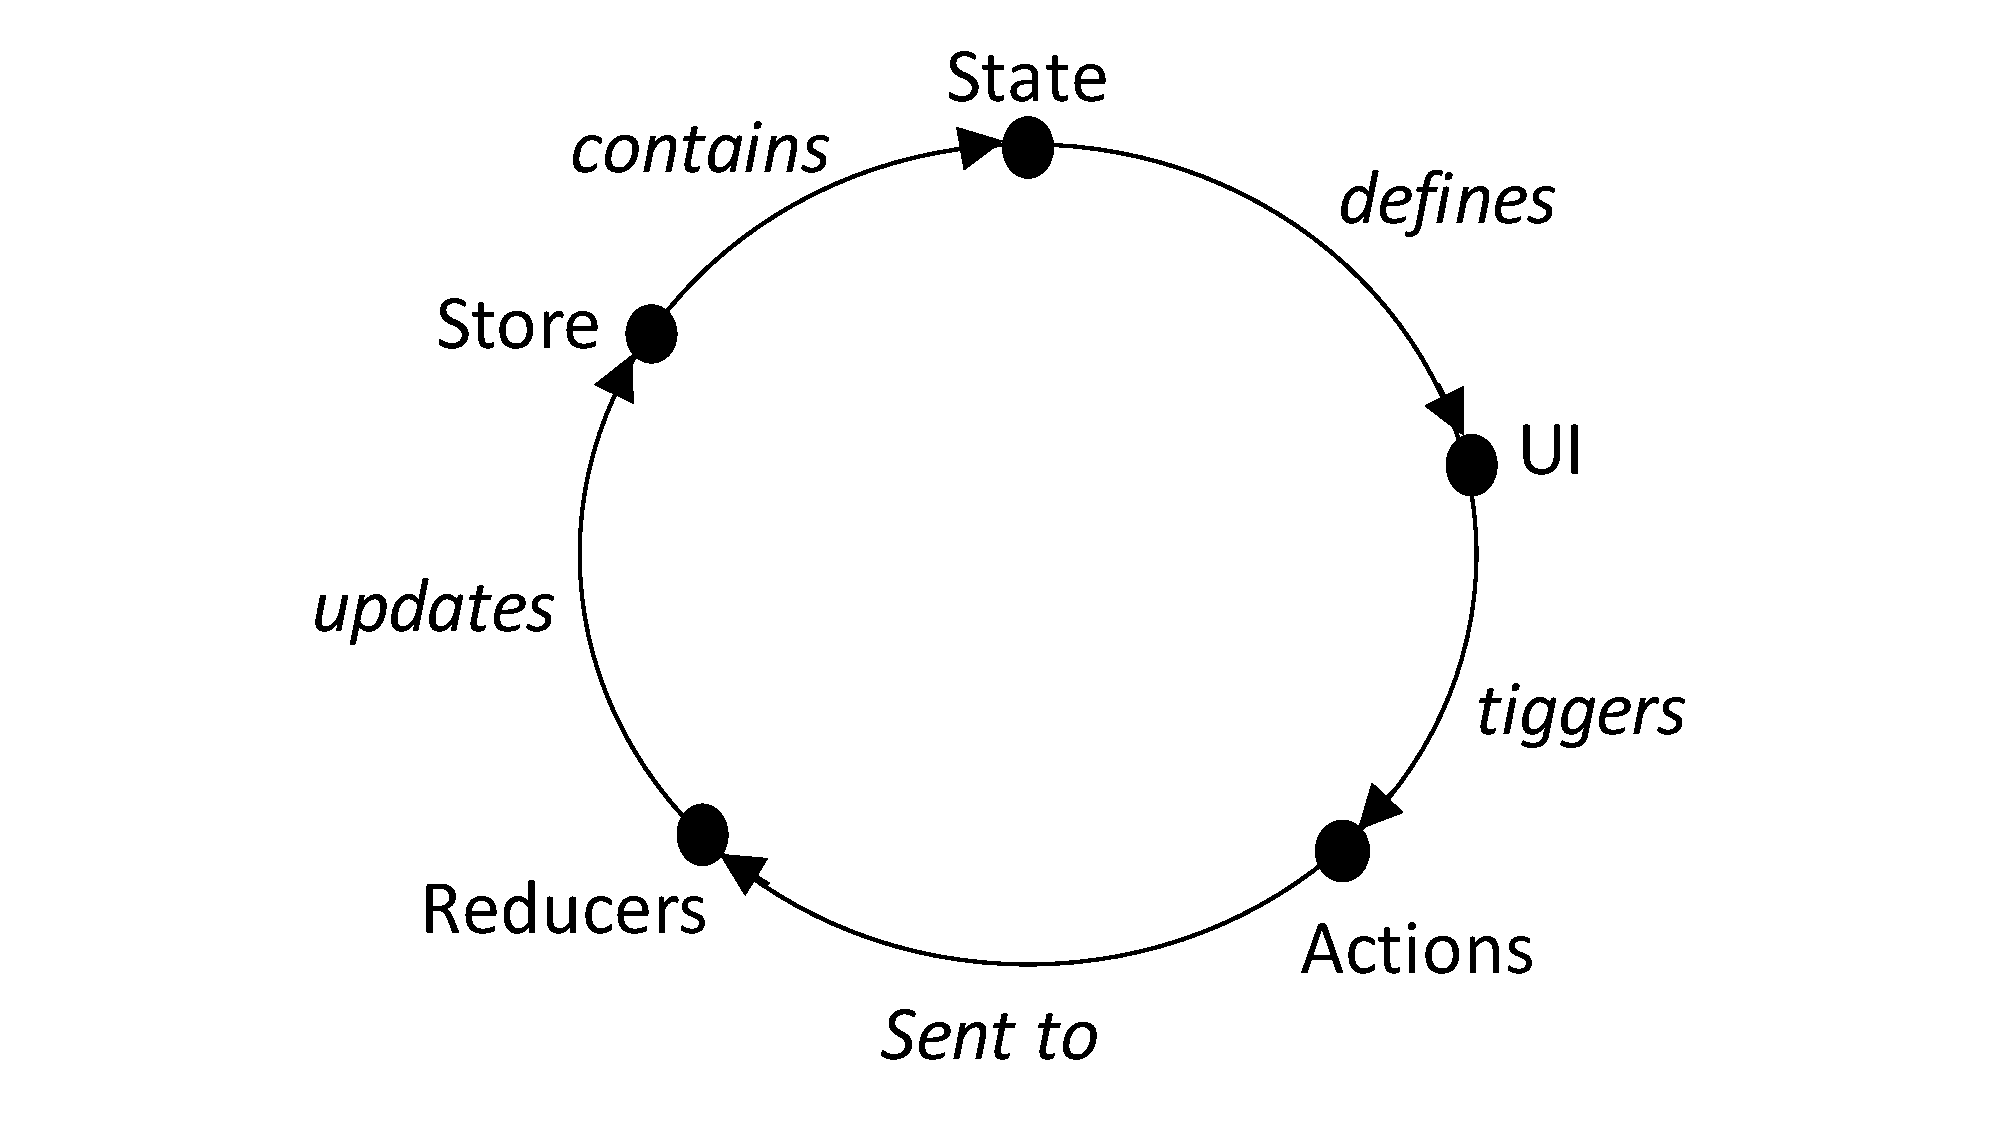
\includegraphics[width=0.5\textwidth]{figs/actions-states}
	\caption{Web client actions and states cycle}
	\label{fig:actions-states}
\end{figure}


Integrating Firebase was one of the most complex tasks because even though the documentation is excellent, there is not enough information on how to integrate Firebase with React and Redux. When we started, our app using only React, everything was handled by functions inside the components. However, because of Redux nature of pure functions Asynchronous calls where a struggle for us. That's why we needed to add a middleware called Redux-thunk ~\cite{46rtrtet}. This is another library widely used by the React Community. However, there is also another one gaining popularity called Redux-saga ~\cite{5656ry} which solves the same issues, doing asynchronous calls inside Redux, that is, fetch and update Firebase whenever an action is dispatched via Redux.

Previously we mentioned how we needed to use Babel to compile our code because of the new Arrow Functions and the \textit{this} keyword. With Firebase, some of the methods didn't work as expected inside React. After much research, we finally found an explanation of this behaviour on StackOverflow which told us that with React and Firebase you had to either “bind” this keyword or use a fat arrow which does this automatically for you. At first the arrow function looked intimidating, but it was less boilerplate code for the rest of the app, so we decided to use this newer feature inside JavaScript and fix the babelrc file accordingly. 

Once we got this issue solved we got on speed, we were getting all the information from Firebase as we needed. The first part was fetching the conversations from Firebase. We used some sample data following the structure we mentioned before. With Firebase, we fetched all the conversations that the loggedUser had in their conversations object. This was one of the most important highlights of our project, because as opposed to a regular SQL Database, there is no such thing as “SELECT * FROM Conversations where conversationID in (SELECT Conversations FROM User WHERE User = “X”)” With Firebase we had first to read the loggedUser, which by that time was a hard-coded “uid” which is the Id that Firebase gives to every new registered user. After that, we needed to fetch all the conversations from that User. And when we finally got those conversations in the same step we needed to fetch all of to the Conversations of the Conversation reference object that were the same as the User’s. This code was really hard to achieve, so we are really proud we got it:


\begin{figure}[ht]
\centering
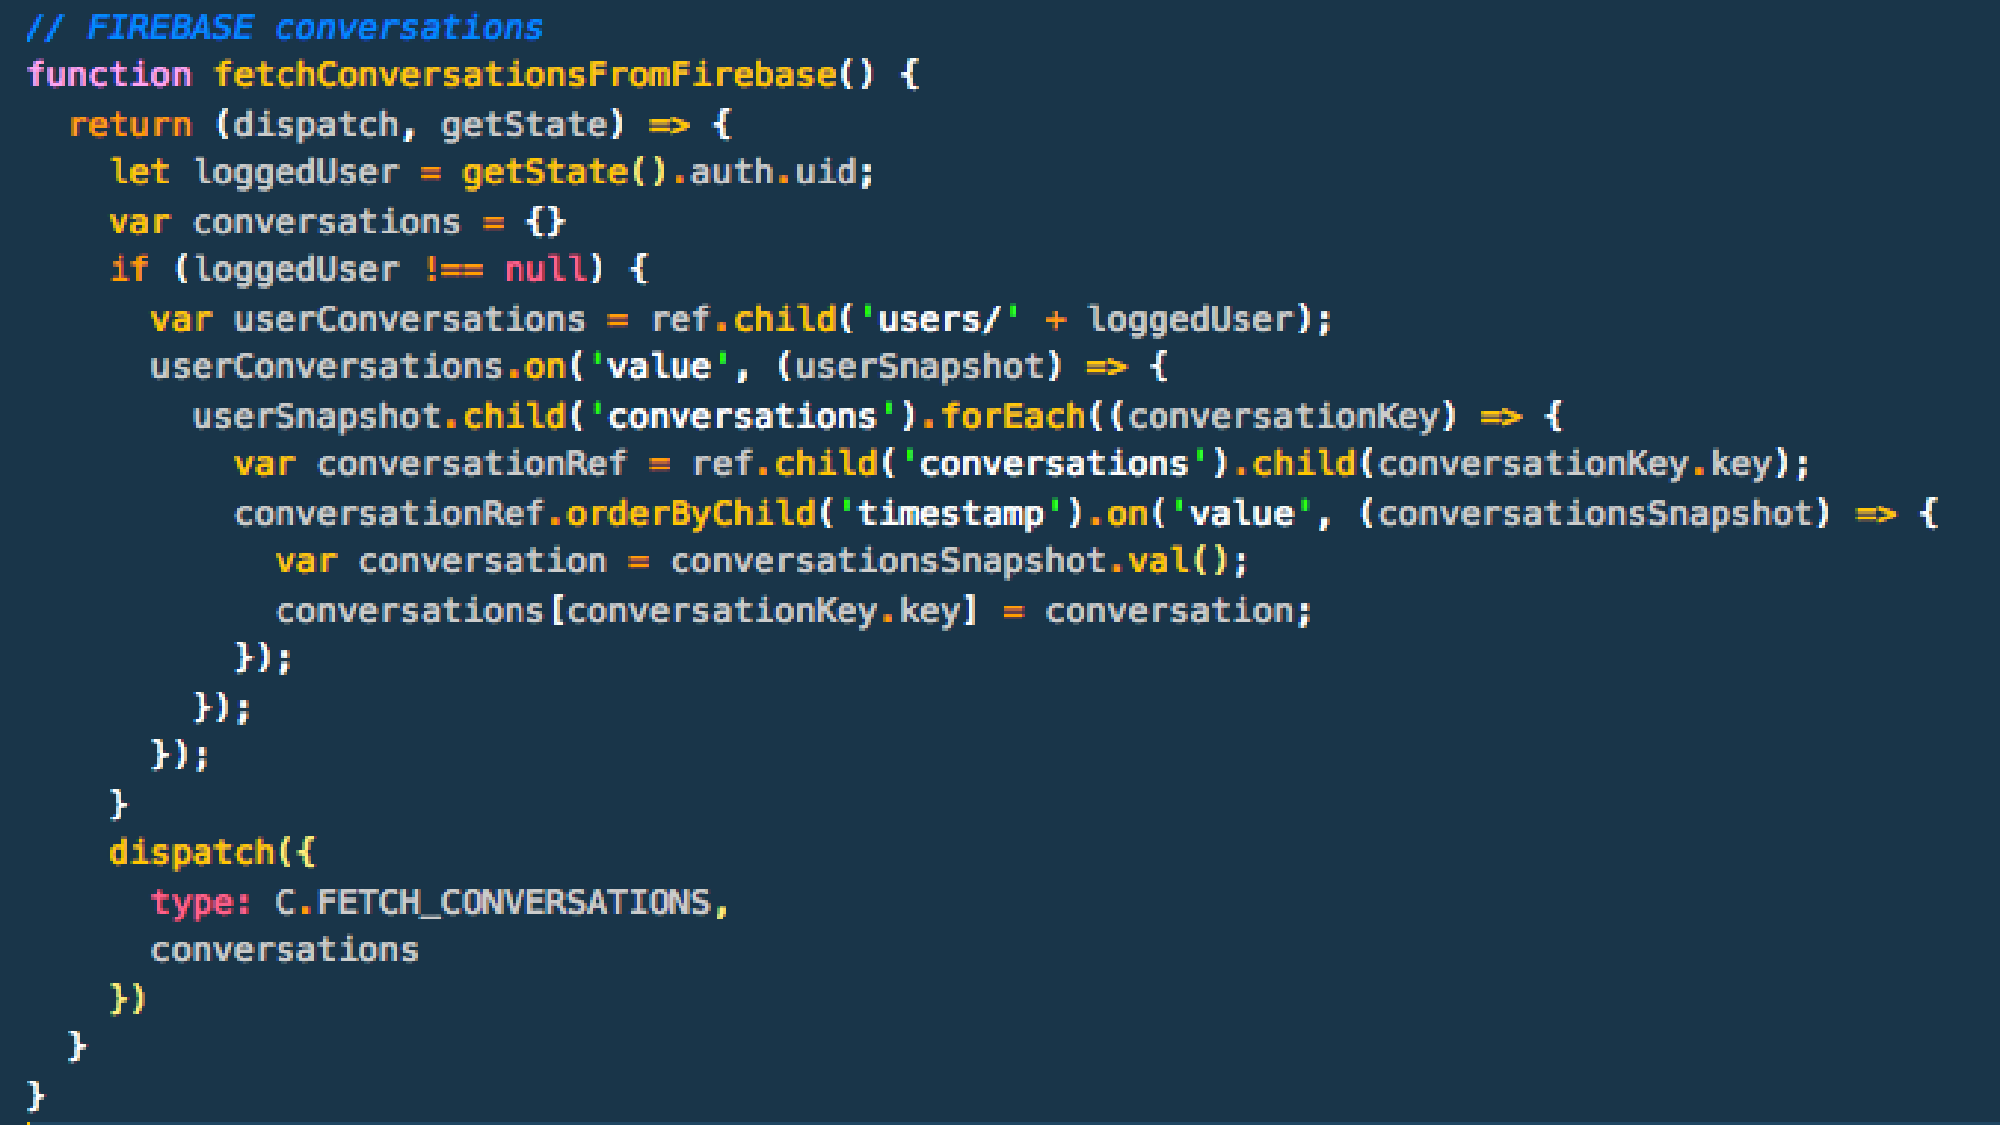
\includegraphics[width=1\textwidth]{figs/Fetch-conversation}
	\caption{Fetch conversation from Firebase}
	\label{fig:Fetch-conversation}
\end{figure}

This was difficult and we wasted a lot of time on learning how to do this. A lot of the Firebase documentation recommends doing a flat database structure precisely because of this, but we didn't quite get the concept of NoSQL databases until we stumble in a post  ~\cite{tutyuty}  which mentions denormalization, a concept that we completely understand the opposite way when learning about relational databases.

With Firebase a lot of the back-end code gets done on the client. To create a new user on Firebase, we needed to register in Firebase, after that, we needed to create the user inside the Users database and make sure to validate the information before adding it to the database. The back-end contains validation rules, however most of them are handled on the front-end. 

For the Participants JSON, we needed to get the Sender and the Receiver id. After that, we created a Conversation Key using Firebase Database Push method which gives the developer a unique key. After that, we added both users to the participant’s object as well as the conversation key to each of the Users object. This kind of seems repetitive but that’s one of the main reasons why Firebase is so fast. Because it only stores simple objects of string data.

The Messages functionality was the most intriguing and interest for us. We wanted to feel like a professional application, that's why we grabbed a lot of inspiration from the WhatsApp Web Client. We even created our bubbles inspired by theirs. Even though CSS is just a styling language it also gave us some lessons.  

It was a little bit complex to learn how to add new messages to the Conversation inside the Messages dictionary, again, it sounds counter intuitive but it did work as intended, we erased some of the sample information inside our Testing Firebase App, however we learn a lot in the process. Adding new messages was one of the most complex tasks, first we needed to get a new key from Firebase. Then if the conversation didn't exist we needed to create it. However, if it existed, we needed to get it from the Participants dictionary. The dictionary that contained both the sender and the receiver was the conversation that needed to get a new message. Again, this was another tricky part that we are proud of having solved.

Some remarks of our software development experience are also that the community in stack overflow and other IRC channels, were helpful. Also, there is a lot of people out there showing their contributions and doing open source code. That excites us a lot and makes us feel more challenged for the future.

Our conclusions for the implementation of the Web client are that we are very happy that we got the minimum functionality working, we wanted to do more as we showed on our initial timetable, however we now feel more experienced and we learned by firsthand the joy of developing with React. Which sounds like in the future is going to keep being useful (see React Virtual Reality ~\cite{4545etet}).


\subsection{Android Implementation}

As new programmers, we started by looking at existing Android messaging apps that use Firebase as a back-end so we could take ideas on how to start. There is a course in Udacity made by Google that makes a basic chat (all to all) that we used as reference for our app ~\cite{4664rtyrtr67}.

Later on, we found out that this app was very different to what we needed. We needed a different database structure to be able to map each message to the appropriate conversation. With this came many complications. We had to change the whole structure of our program! We tried changing our code, but we found out that it was a hard task so we decided to start a new project from zero because it would be easier.
We had many problems during the way but only one that we were not able to fix. We didn't manage to append a new message to the previous list of messages of a specific conversation.

We think that the steps to do it are as follow, but we don’t know how to implement them:

\begin{itemize}
	\item Get the user id (the key) of the sender [Done].
	\item Get the user id of the receiver.
	\item Search inside each “participants” children if the userid of the sender and receiver match the keys stored with a value of true.
	\item Get the “participants” children key that found before. This is the key for the conversation for the 2 participants.
	\item Go to ``messages" $\rightarrow$ ``key-found-in-previous-step" $\rightarrow$ append the message.
\end{itemize}

The android app doesn't have a register functionality because the priority was to solve the previous problem and then tackle the next one. We can not display the senders username in the chat room, so we display the userid instead.
We have different classes in our app:

\begin{itemize}
	\item \textbf{Chat}: Containing the instances of sender, receiver, senderUid, receiverUid, message and timestamp.
	
	\item \textbf{Chat-room}: This class is in charge of what happens inside the conversation. It already knows who the sender and receiver of the new message are and it finds out what were the previous messages of these 2 participants and appends the new message. 
	
	\item \textbf{LoginActivity}: This class is in charge of the log in process. In contrast with the other clients, a new user can only sign in and not sign up. The user can only sign in with an email and a password.
	
	\item \textbf{MainActivity}: This class is responsible for connecting everything in the app. It has many methods including a method that is responsible for getting and showing all the open conversations with the different users, a method that converts the receiver uId to the receiver name so it can display the name in screen.
	
	\item \textbf{User}: Class containing the instances of name, userId and email.
	
	\item \textbf{UserListActivity}: Class containing a method to get all the users from Firebase.

	\item \textbf{UsersArrayAdapter}: Special class made for android to be able to map a list of users to a list view. We display thanks to cellprototype.xm
\end{itemize}




\subsection{Testing}

For the test, we were inspired by the verification and validation model (V- model), which is based on the relationship between each phase of a software development life cycle, were and associated testing phase is added.   The next figures summarise each phase of the methodology, which also is an integral part of our developed philosophy. 

\begin{figure}[ht]
\centering
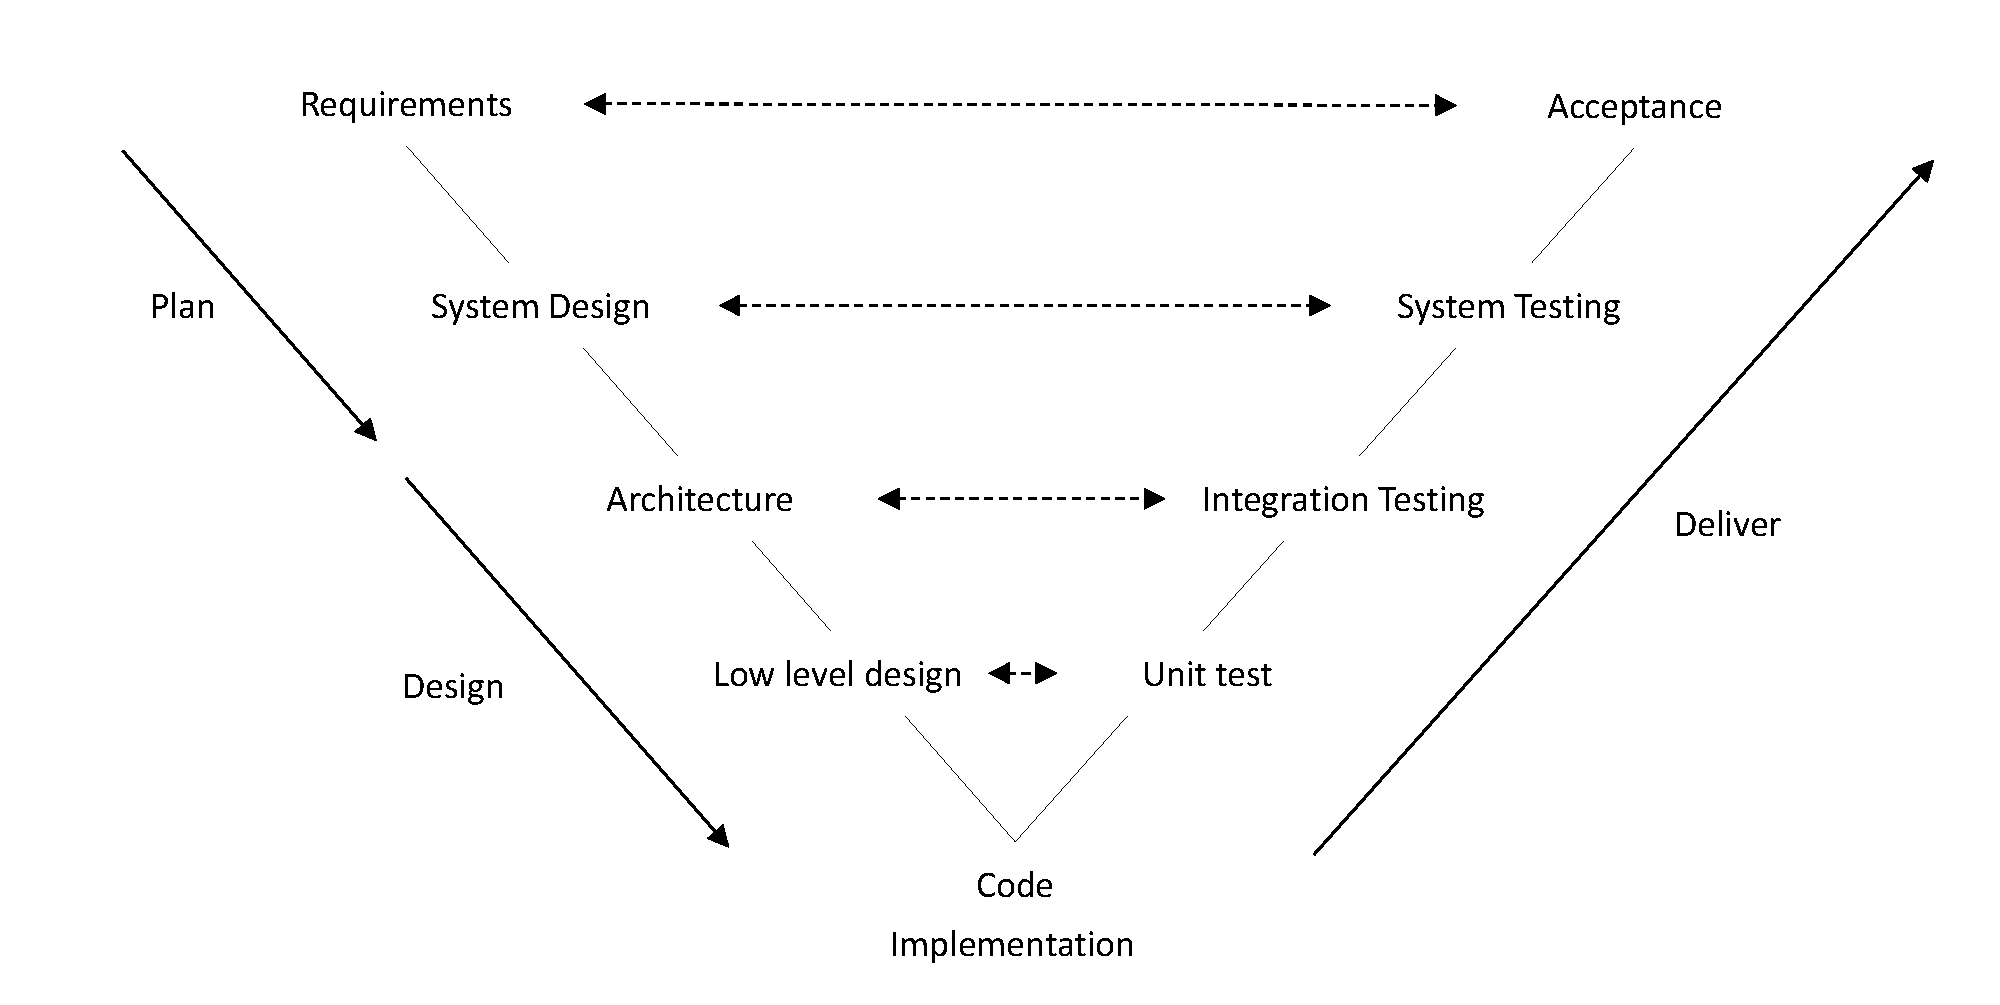
\includegraphics[width=1\textwidth]{figs/testing-met}
	\caption{Test foundation Methodology}
	\label{fig:testing}
\end{figure}


Despite we are aware of the agile test methodology model (where each little division or task of software is tested while developing ~\cite{rtyeteey}), in our case this was not at all useful, considering that we have a priority requirements list. This means that the divisions of our software, as well tour architecture, changes according with our learning curve across this project. Thus, our initial plan or division of the software were extremely dynamically to adequately divided since the beginning. In fact, we can say that this is the main challenge our group face.

The next table presents the results of the testing process. An iterative process was conducted to guarantee a proper integration of the different clients.  Also, this process is challenging, considering that while we are trying to develop each client, at the same time we must be aware the whole structure of the system.  


In addition to the previous methodology, we can also have said that our testing process was iterative across the development in the following sense: 

Initial Testing.	Initial testing was the first test conducted on the application. The testing process began with the testing of the login unit/page that was demonstrated    during the initial presentation. At that point the testing was platform specific. There was no need for testing together across other platforms then. However, as the development progressed, our testing methodology was modified. 

Development Phase Testing.	These are the testing conducted through the development phase of the project.  The testing done during the development phase was such that the codes were shared amongst the team as soon as they were observed to be working and deleted or overwritten once it was found not to be working or not to meet our desired end. The testing was done intermittently as the project was being developed. The result of each test determined progression to the next phase. No member of the group was dedicated as a test engineer neither was any sub-team assigned the responsibility of testing the software. However, as each sub-team was working on its project, the test was also going on. Whoever was writing the code was a test engineer in his own right. Then when the team meets, the codes were run across platforms to query its compatibility and flexibility across platforms. The team members from the different platforms then criticise the codes based on their observations (Red Teaming) and suggested necessary modifications.

Final/Integration Testing. The final test is an integrated testing at the end of the project.  The final testing was done to ensure that all the users were able to carry out one to one conversation across the three clients’ platforms. At this stage, we encountered a challenge of the inability of the three clients’ bases to communicate directly with each other. However, the database structure was re-examined and the sub-teams developing the clients were made to restructure their back-end to follow the same format. Then, the inter-communications issue across the three platforms was resolved.   

\begin{figure}[ht]
\centering
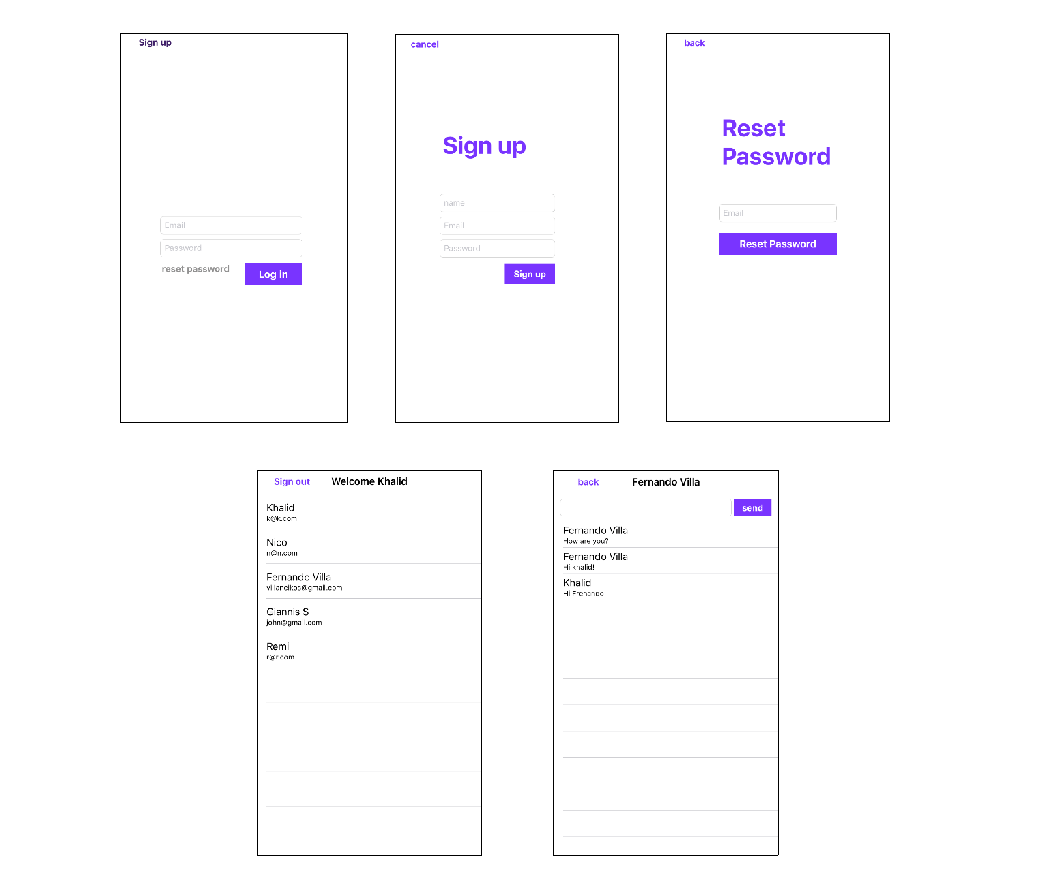
\includegraphics[width=1\textwidth]{figs/IOSscreen}
	\caption{iOS Screenshots }
	\label{fig:IOSscreen}
\end{figure}

\begin{figure}[ht]
\centering
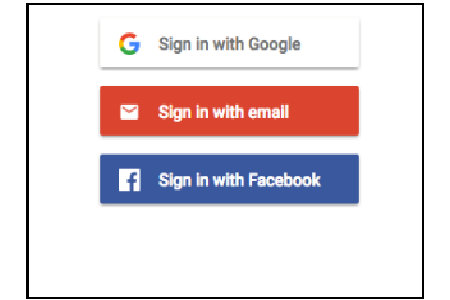
\includegraphics[width=0.3\textwidth]{figs/weblog}
	\caption{weblog }
	\label{fig:weblog}
\end{figure}

\begin{figure}[ht]
\centering
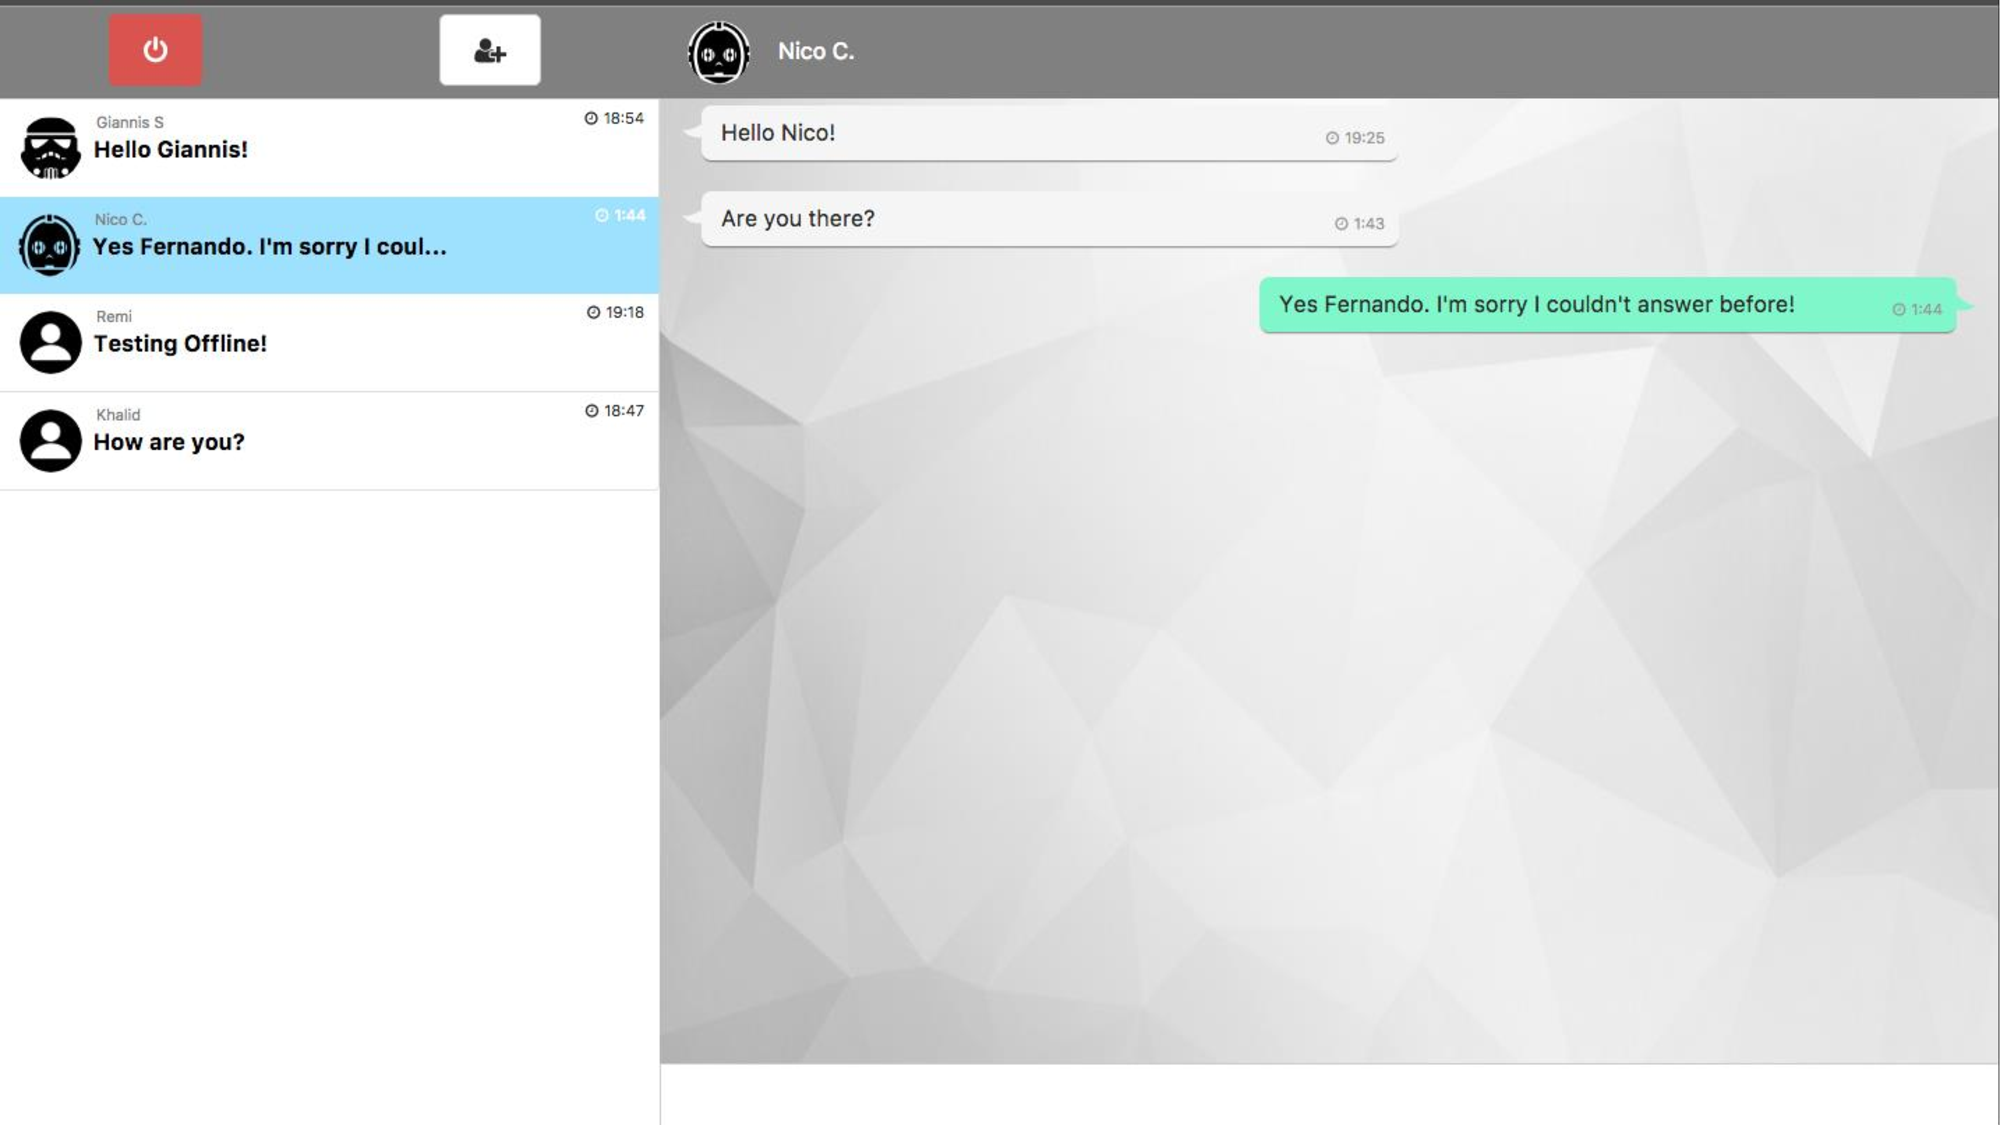
\includegraphics[width=1\textwidth]{figs/Chat-sample-Conversation}
	\caption{Chat-sample-Conversation }
	\label{fig:Chat-sample-Conversation}
\end{figure}

\begin{figure}[!t]
\centering
\subfigure[Main Screen]{
	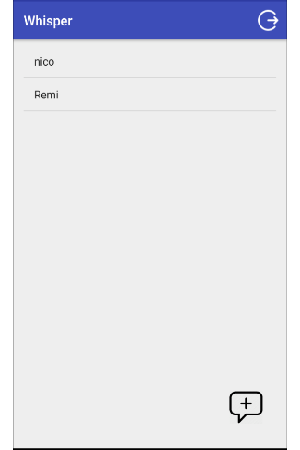
\includegraphics[width=0.3\textwidth]{figs/mainscreen}
	}
	\subfigure[Chat]{
	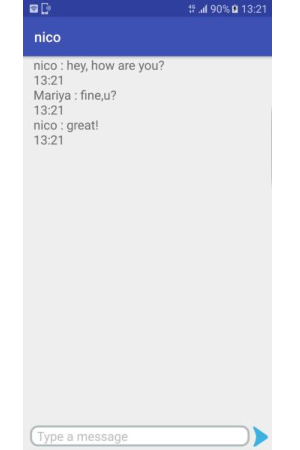
\includegraphics[width=0.3\textwidth]{figs/chatandroid}
	}
	\subfigure[Create New Conversation]{
	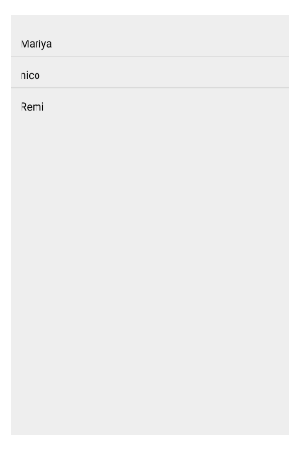
\includegraphics[width=0.3\textwidth]{figs/Newconversation}
	}
	\subfigure[Create New Conversation]{
	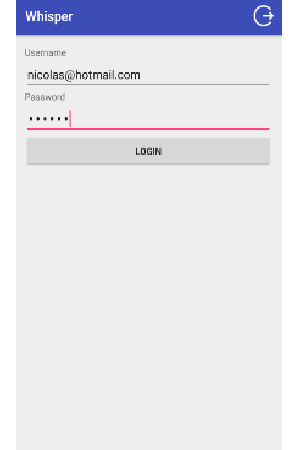
\includegraphics[width=0.3\textwidth]{figs/loginandroid}
	}
	\caption{Android Screenshots}
	\label{fig:android}
\end{figure}

